\subsection{\LARGE Tools and Dependencies}

    Before we get to implementation of project, we will talk about development environment, tools and libraries we used.

    \subsubsection{\textbf{\large Visual studio 2022}}

        Microsoft IDE which makes handling and debugging multiple complex projects much easier.

    \subsubsection{\textbf{\large Premake}}

        Open source tool for generating cross platform build files for Visual Studio

    \subsubsection{\textbf{\large Tigraf Engine}}

        Graphics Engine which we will use as core of a whole project. From visualisation to speeding up learning algorithms.

\subsection{\LARGE Classes and Initialization}

    \subsubsection{\textbf{\large AppLayer}}

        The Tigraf Engine core operates by sending events, updates, and other actions through layers. In this project, only one layer is required, referred to as the AppLayer. This layer includes the declaration of the necessary functions for the project:

        \hfill
        
        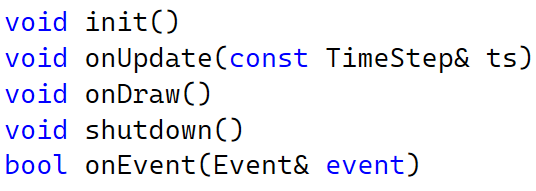
\includegraphics[width=3in]{resources/Layer.png}

        \begin{itemize}
        
            \item \textbf{init}

            Objects are instantiated here and shaders are loaded from memory.

            \item \textbf{onUpdate}

            Here we update the necessary objects and data structures. Most important things here are physics simulation step and neural network which updates movement.

            \item \textbf{onDraw}

            Rendering commands are called from this function. It is used for rendering background, grid and loaded shapes.

            \item \textbf{onEvent}

            All operating system, window and user events are handled here.

            \item \textbf{shutdown}

            This function is mainly used to free memory.
            
        \end{itemize}

    \hfill
    
    \subsubsection{\textbf{\large Shape}}

        This structure defines a look of an entity which is learning how to walk.

        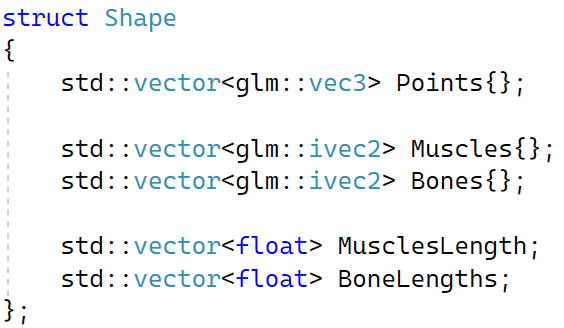
\includegraphics[width=3in]{resources/Shape.png}

    \hfill

    \subsubsection{\textbf{\large ShapeLoader}}

        This class comprises static methods for loading the shape from memory. The points are stored as "points" where each line of text represents a point, with the coordinates separated by spaces. Similarly, there are sections for "bones" and "muscles" where each line of text contains two indices.

    \hfill

    \subsubsection{\textbf{\large ShapeRenderer}}

        This class serves as the main location for methods related to initializing and transferring all required project data to the GPU. The ShapeRenderer class offers a range of static methods for handling tasks such as rendering, simulation, and learning. These methods are called from the AppLayer.

\subsection{\LARGE A closer look into the ShapeRenderer}

        The engine core of the program provides various data structures, including buffers, for the ShapeRenderer to utilize in order to transfer data to the GPU. As the primary objective of this project is to optimize performance, a majority of the buffers employed are RWBuffers, which are enabled for both reading and writing on the GPU side. This approach eliminates the need to constantly copy data to the CPU, thus removing the largest bottleneck in the system. The buffers utilized in this program are listed below for reference.

        \begin{itemize}
            
            \item{\textbf{PosVelBuffer}}
                is used to store positions and velocities of each point for each instance.
                It is modifiable by shaders.

                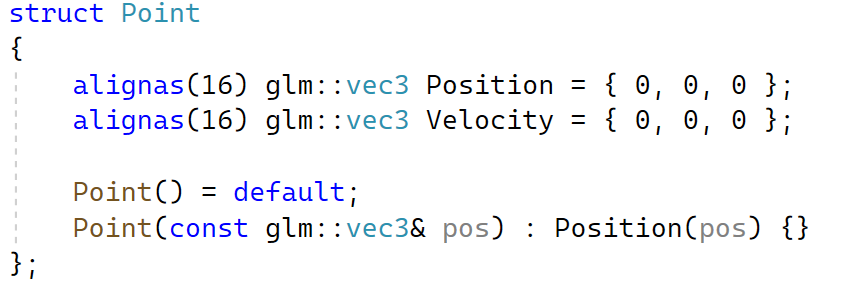
\includegraphics[width=3in]{resources/Point.png}

            \item{\textbf{LengthBuffer}}
                is used to store muscle lengths for each instance.
                It is modifiable by shaders.

            \item{\textbf{LayerBuffer}}
                is used to store 3-layered neural network for each instance. It is filled randomly and it is also modifiable by shaders. The second largest performance bottleneck in the system is identified within this buffer. During the process of instantiating the next generation, the GPU threads require access to data from one another, which necessitates the use of coherency and barrier bits. To address this issue, a solution was implemented by duplicating the buffer and utilizing both copies in a zig-zag fashion. This approach eliminated the need for synchronization throughout the entire project, resulting in a significant improvement in performance!

            \item{\textbf{StatsBuffer}}
                is used for storing statistic data such as instance count, movement distance, mean and variance.
                It is modifiable by shaders.

            \item{\textbf{FitnessIndicesBuffer}}
                is used for storing the fitness of each instance each episode.
                It is modifiable by shaders.

                \item{\textbf{ShapeDataBuffer}}
                is used to store immutable information of shape such as points count, muscles count, default muscle and bone lengths.
                It is a read-only buffer.

                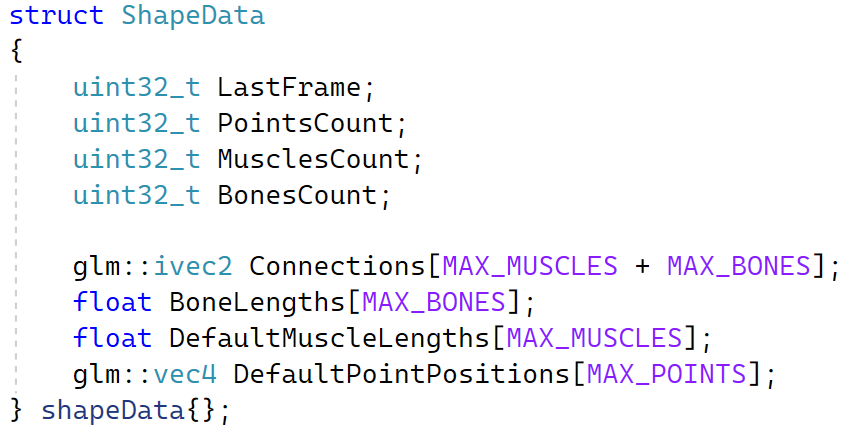
\includegraphics[width=3in]{resources/ShapeData.png}

            \item{\textbf{ShapeVertexBuffer}}
                will be used for storing pairs of indices which form connection and a boolean value saying whether it is a muscle or a bone.
                It is immutable and it will be used for drawing.
                
        \end{itemize}

        \hfill

\subsection{\LARGE Examining the Shaders}

        Apart from initializing buffers, we few compute shaders are also loaded into a memory:

    \subsubsection{\textbf{\large ShapeShader}}
        Used for drawing certain amount of instances. It uses points and connections from \textbf{ShapeVertexBuffer} and \textbf{ShapeDataBuffer} to visualize shape. 
        Depending on the instance id, it connects certain points. With help of normals, tangents and bitangents it creates cuboid limbs and adds lighting effect to each surface.

    \subsubsection{\textbf{\large PhysicsCompute}}
        Used for doing a physics step. It modifies \textbf{PosVelBuffer}.
        Takes previous positions and velocities and modifies them using gravity, damping, springs, friction and floor force. Additionally, it fills \textbf{FitnessIndicesBuffer} on the last iteration of current generation.

    \subsubsection{\textbf{\large GeneticCompute}}
        Used for controlling muscle and shape movement. It modifies the \textbf{LengthsBuffer} by reading the \textbf{LayerBuffer}. It runs through a neural network for each instance with the input of absolute position of the first point, absolute velocity of the first point, all positions relative to the first point and all velocities relative to the first point. The output is new muscle lengths for that instance.

        Output will be new muscle lengths for that instance.

    \subsubsection{\textbf{\large EvolutionCompute}}
        Used for rewarding and reproducing fit instances and, of course, \textbf{murdering} bad instances. It modifies \textbf{LayerBuffer} based on \textbf{FitnessIndicesBuffer}.